\chapter{System (or Project) Design and Architecture}
    \section{Use Case Diagram}
    The Use Case Diagram of the prepared inference system.
        \begin{figure}[h]
        \centering
            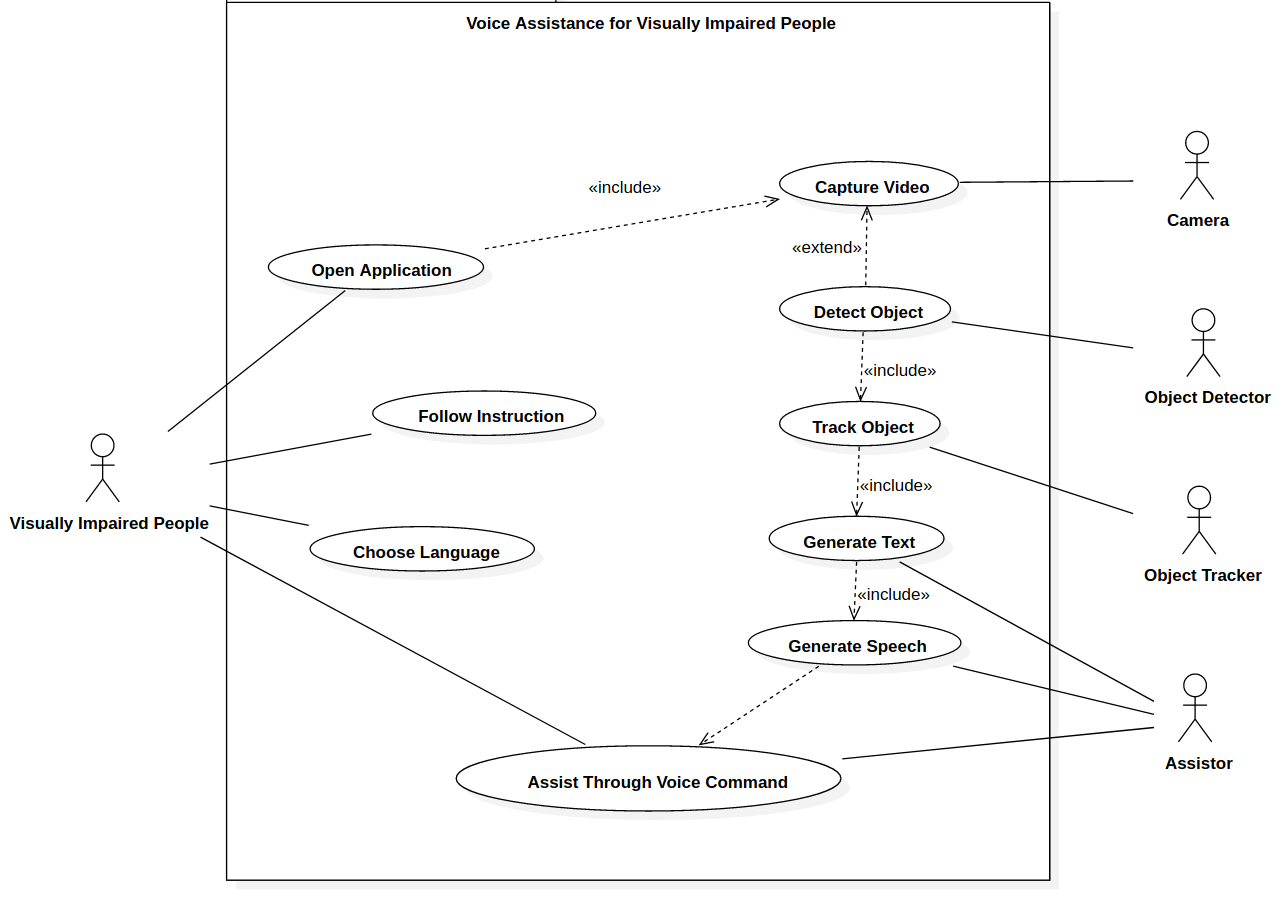
\includegraphics[width=1.0\textwidth]{img/Final_UseCase.png}
            \caption{Use case Diagram}    
        \end{figure}
    \pagebreak
    \section{Context Diagram}
    The Context Diagram shows the top level picture of the system.
    \begin{figure}[h]
            \centering
                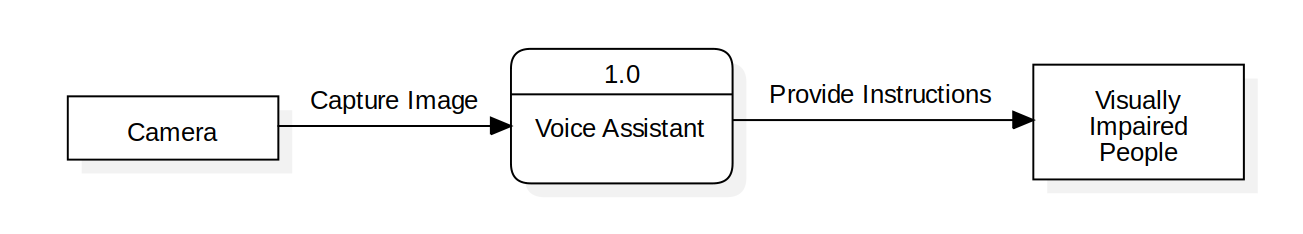
\includegraphics[width=1.0\textwidth]{img/context_Diagram.png}
                \caption{Context Diagram of Inference System}    
            \end{figure}
        \section{Data Flow Diagram}
    The Data Flow Diagram shows the flow of the data between the subsystem of the inference system. The Data flow Diagram of the inference system is shown below:
            \begin{figure}[h]
            \centering
                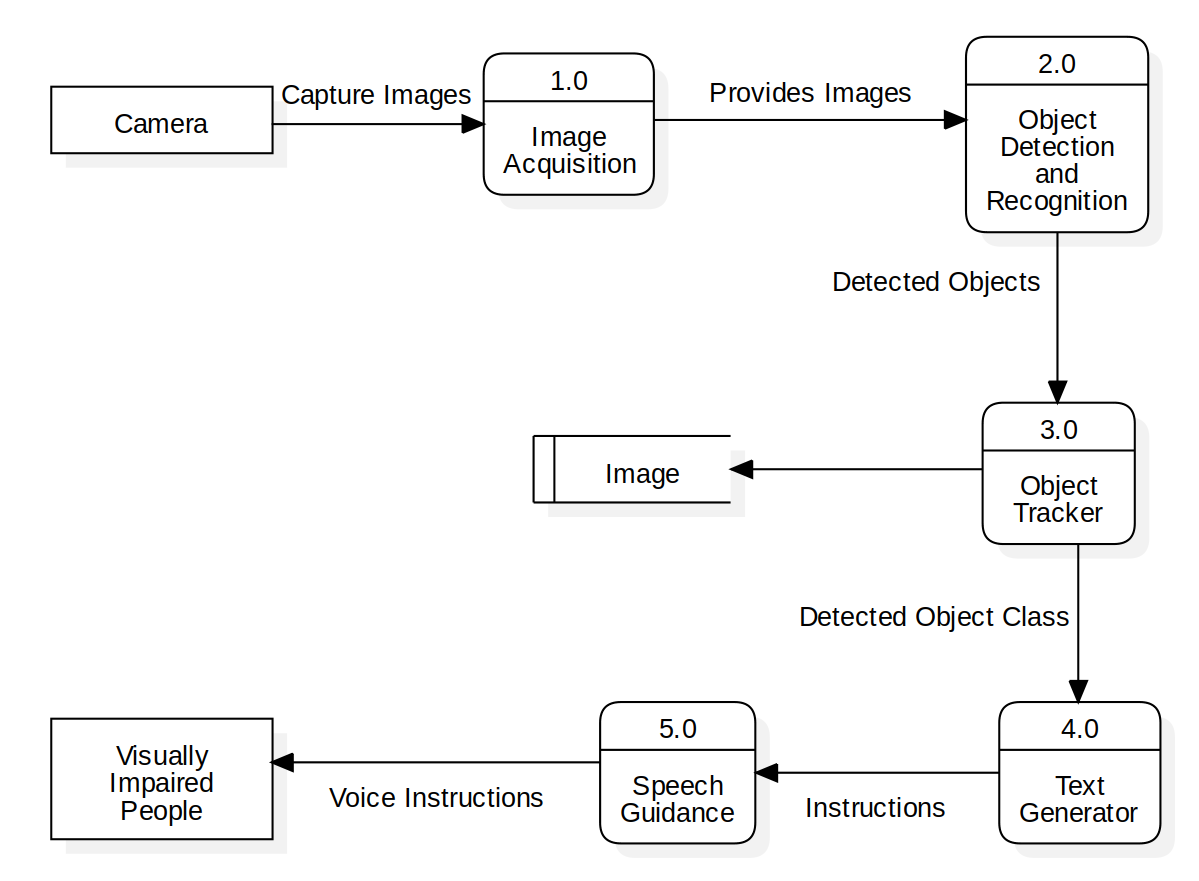
\includegraphics[width=1.0\textwidth]{img/Final_DFD.png}
                \caption{Data Flow Diagram of Inference System}    
            \end{figure}
    \pagebreak
    \section{Sequence Diagram}
    The Sequence Diagram shows the flow of the process in between the subsystem. And the state when the subsystem are active and when the sub system are passive. The Sequence Diagram of the inference system is shown below:
            \begin{figure}[h]
            \centering
                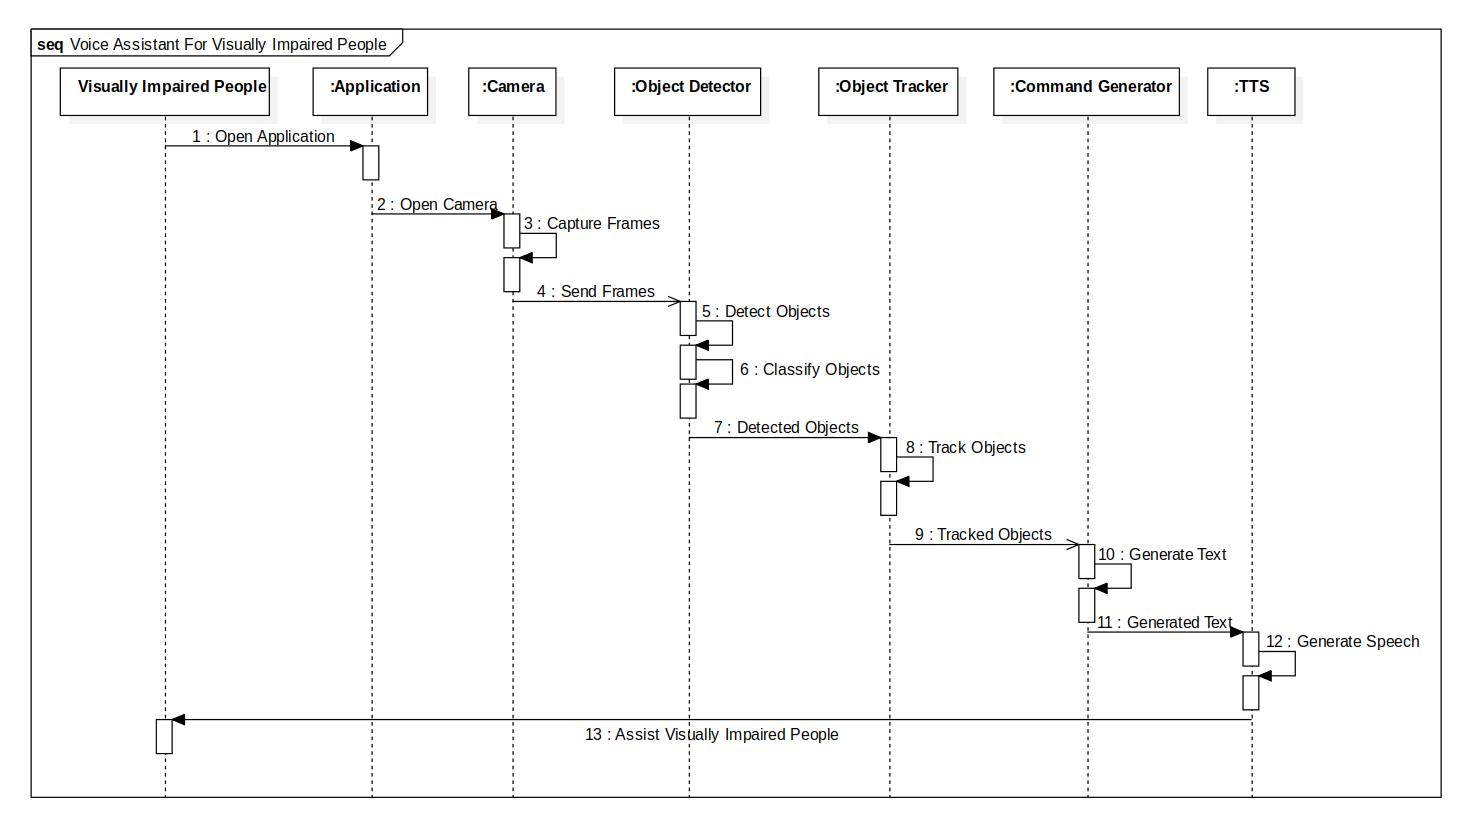
\includegraphics[width=1.0\textwidth]{img/Final_Sequence.png}
                \caption{Sequence Diagram of Inference System}    
            \end{figure}
    \pagebreak
    \section{Schedule (Gantt Chart)}
        \begin{figure}[h]
                \centering
                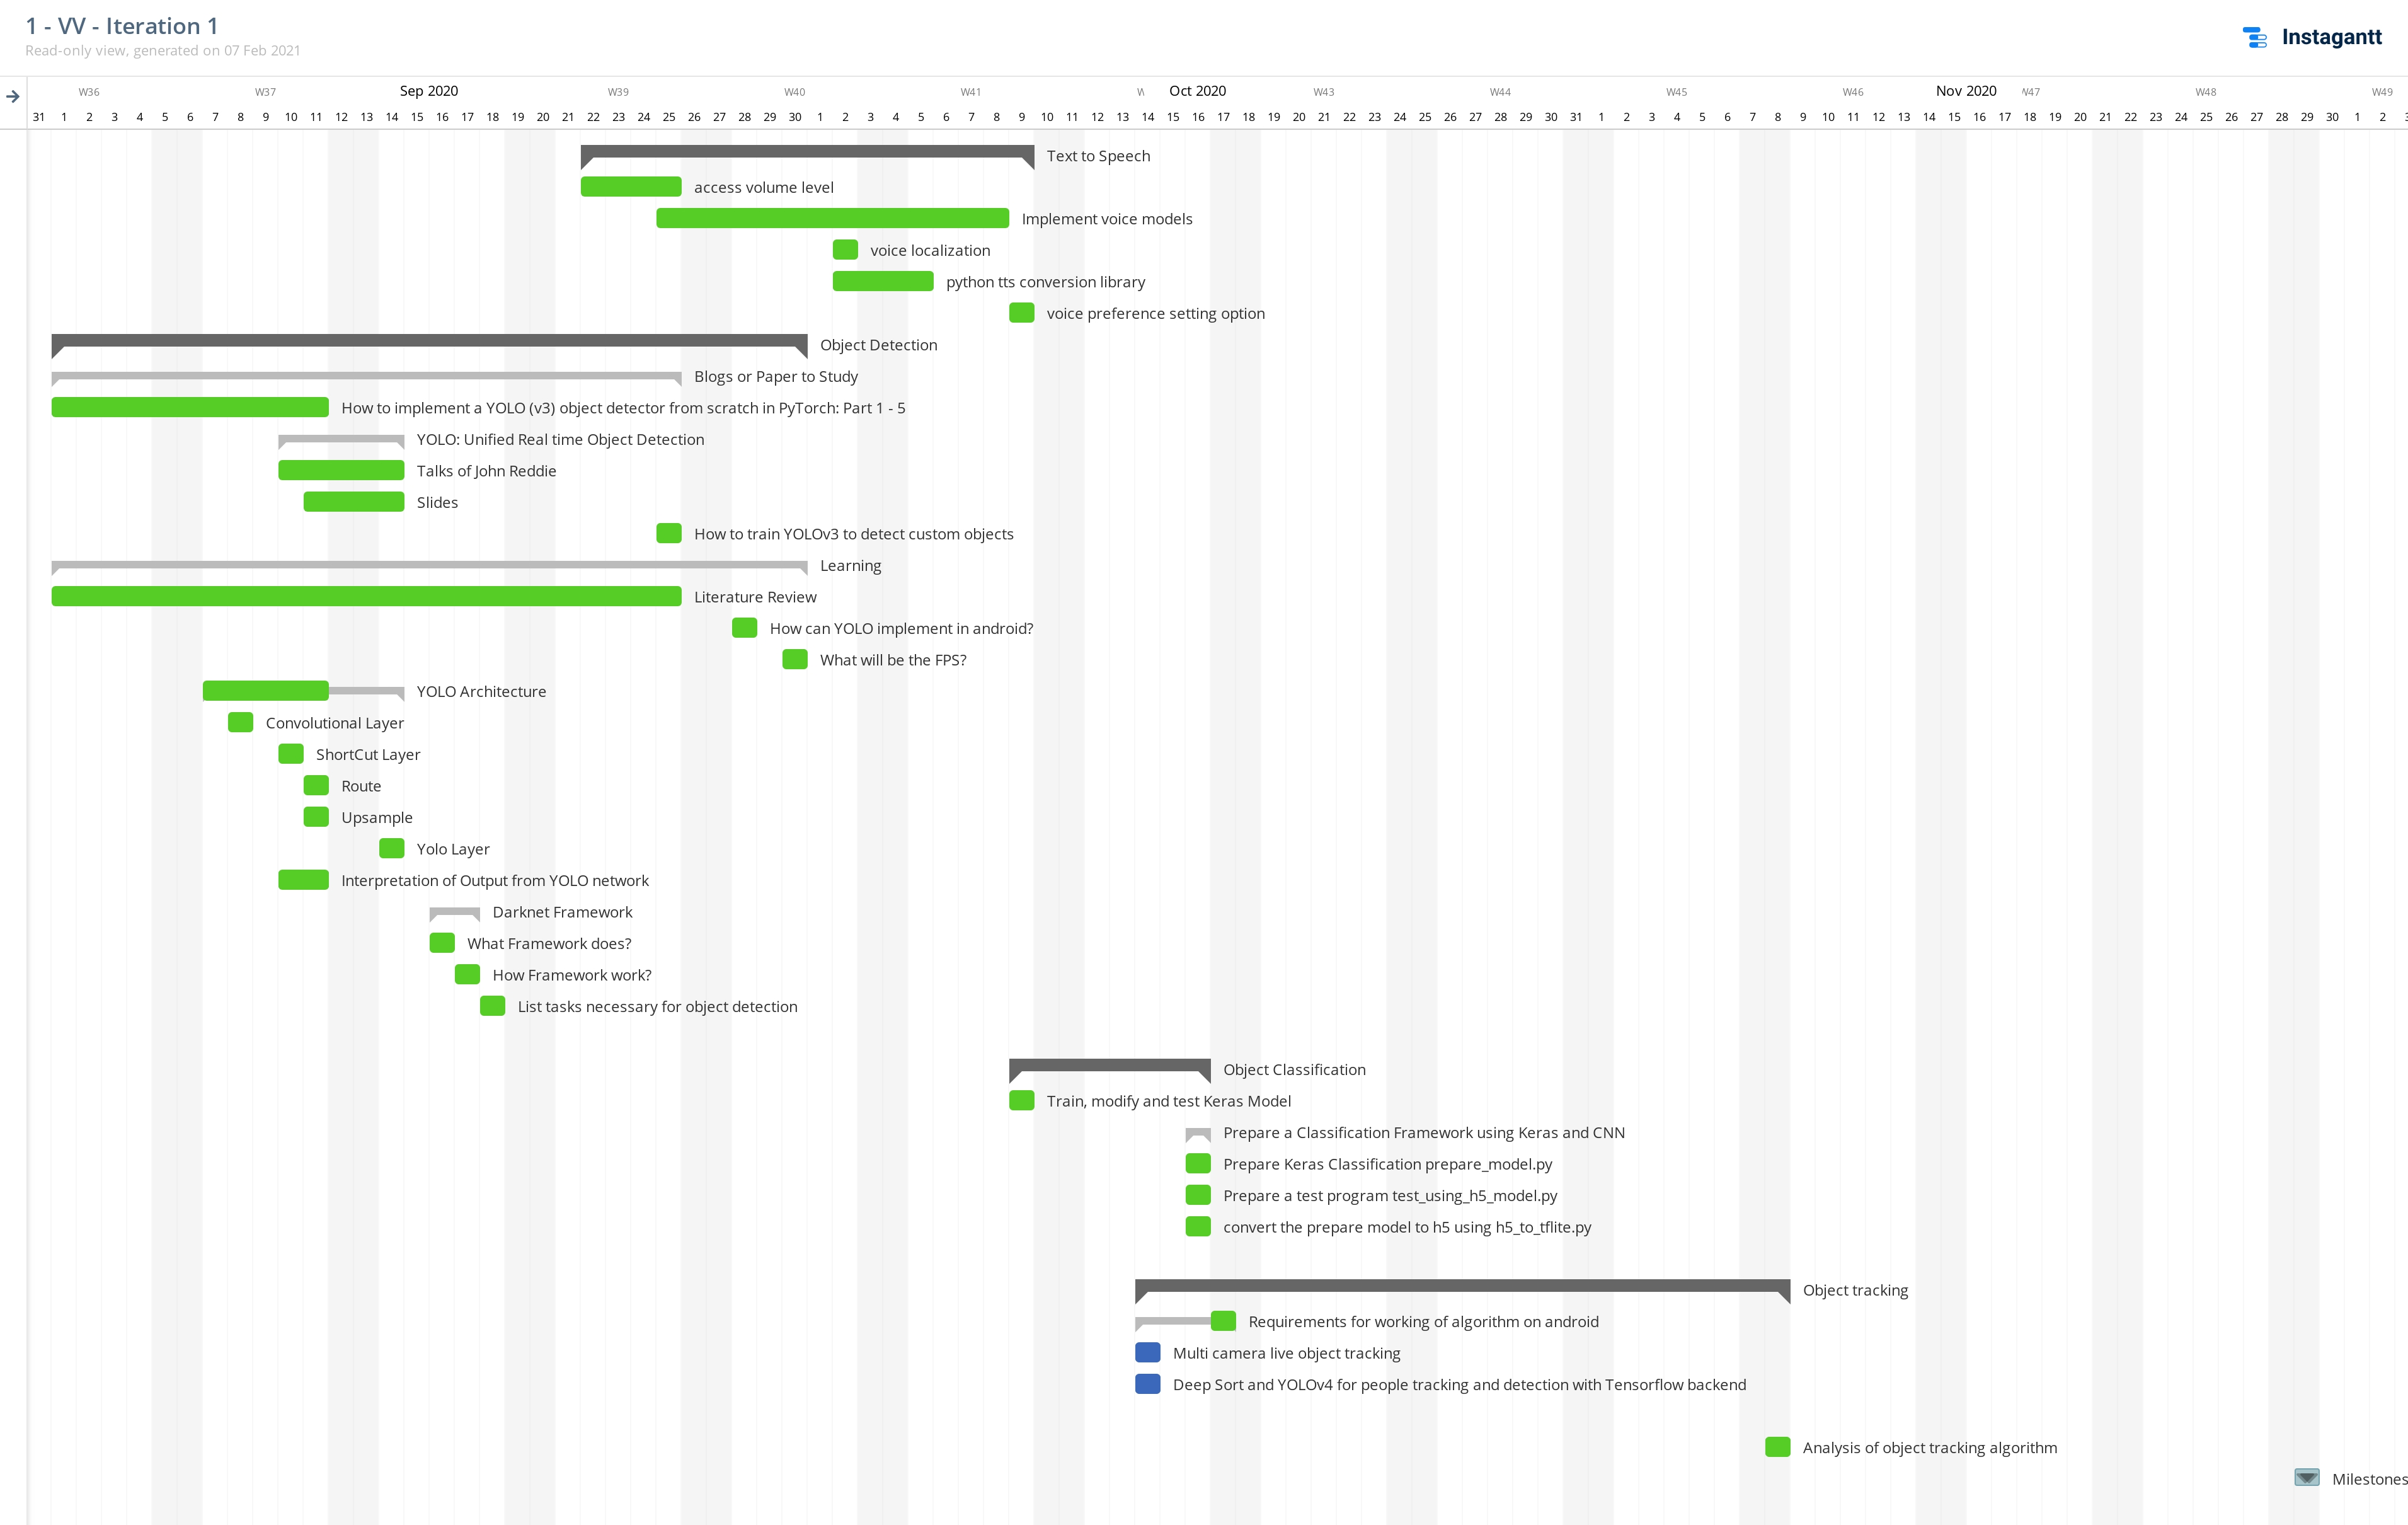
\includegraphics[width=1.0\textwidth]{img/gantt_chart.jpeg}
                \caption{Gantt Chart}
                \label{fig:Gantt Chart}
            \end{figure}